\chapter{Caso práctico}\label{cap:09caso}
En este capítulo se presenta: \ref{sec:09intro} Introducción al caso práctico, \ref{sec:09huvr} El estudio realizado por el Hospital Universitario Virgen del Rocio, \ref{sec:09atlas} El estudio realizado utilizando ATLAS, \ref{sec:09resultados} Discusión de resultados y \ref{sec:09conclusiones} Conclusiones.

\section{Introducción} \label{sec:09intro}

Este capítulo pretende demostrar la relevancia de OHDSI (Observational Health Data Science and Informatics) y la utilidad de sus herramientas, concretamente el uso de ATLAS para la estandarización y reproducibilidad de los análisis clínicos observacionales sobre bases de datos estandarizadas al Modelo de Datos Común de OMOP. 

Para ello, bajo la tutela de D. Carlos Parra y Da. Silvia Rodríguez (tutores de las prácticas en empresa, véase \ref{sec:03Participantes} ''Participantes del proyecto''), se ha seguido la reproducción de un estudio realizado por investigadores del hospital sobre predicción mediante modelos de ML de efectos adversos en el tratamiento radioterápico de pacientes con cáncer de pulmón. 

Este estudio, se encuentra públicamente accesible en Pubmed en dos artículos, el primero publicado en el año 2019 titulado \textit{''Comparison of Feature Selection Methods for Predicting RT-Induced Toxicity'' }\cite{nunez2019comparison} y el segundo, en 2023 titulado \textit{''Benchmarking machine learning approaches to predict radiation-induced toxicities in lung cancer patients''} \cite{nunez2023benchmarking}. Ambos estudios están también publicados en la ruta \code{Thesis-ATLAS-OHDSI/documentation/pdf/estudioHUVR} del repositorio de github del TFG \cite{vallealonsodc}.

El objetivo es promover el uso de ATLAS para la investigación observacional, reproduciendo mediante ATLAS un estudio que fue realizado sin hacer uso de la herramienta, para demostrar con un caso práctico los beneficios de utilizar la herramienta en términos de reproducibilidad y estandarización.

\section{Estudio realizado por el HUVR} \label{sec:09huvr}

El estudio consiste en la comparación de 300 modelos de ML sobre un dataset de 875 pacientes de cancer de pulmón con el objetivo de predecir los efectos adversos a corto (esofagitis, tos, disnea y neumonitis) y a largo plazo (disnea y neumonitis) que producirá el tratamiento radioterápico sobre estos pacientes. 

\subsubsection{Contexto}

%La base teórica del estudio \cite{nunez2019comparison, nunez2023benchmarking} es que la radioterapia aunque es beneficiosa para el tratamiento oncológico, también causa efectos perjudiciales a corto y/o  largo plazo de forma personalizada según las condiciones de cada paciente. El auge de la medicina personalizada y centrada en el paciente (véase \ref{sec:01Contexto}) ha ensalzado la importancia de realizar una planificación individual para cada paciente, pues cada persona responde de forma distinta a los tratamientos. Por tanto, la gestión individualizada de los posibles efectos adversos es muy importante en la planificación del tratamiento radioterápico, con el fin de facilitar la toma de decisiones entre médico y paciente en términos de calidad de vida y posibilidades de supervivencia.

La radioterapia, aunque beneficia el tratamiento oncológico, puede ocasionar efectos perjudiciales a corto y largo plazo, de forma personalizada según cada paciente \cite{nunez2019comparison, nunez2023benchmarking}. La medicina centrada en el paciente (véase \ref{sec:01Contexto} ''Marco contextual'') destaca la importancia de planificar individualmente cada tratamiento, dado que las respuestas varían entre individuos. Por tanto, la gestión personalizada de los efectos adversos es crucial en la planificación radioterápica para facilitar la toma de decisiones médico-paciente en términos de calidad de vida y supervivencia.

\subsubsection{Objetivo}

El objetivo del estudio es utilizar un conjunto de datos del mundo real (RWD) para facilitar la toma de decisiones clínicas, estudiando para cada efecto adverso del tratamiento radioterápico, el modelo de ML que provee una mejor predicción en términos de precisión del modelo (AUC).

\subsubsection{Datos}

- RWHD

\textcolor{red}{- 875 pacientes del registro s31 y observacion del huvr??}

\subsubsection{Metodología}

Para conformar los 300 modelos de ML se han entrenado y testeado 5 modelos de ML combinados con 10 métodos de selección de atributos (\textit{Feature Selection, FS}) sobre 6 efectos adversos (\textit{outcomes} o \textit{clinical endpoints}), de la siguiente forma: 

\begin{itemize}
    \item \textbf{5 Modelos de ML}. Se utilizaron cinco clasificadores basados en aprendizaje 
    automático: 
    \begin{itemize}[label={--}]
        \item Máquina de Vectores de Soporte (\textit{Support Vector Machine, SVM}).
        \item Vecinos más Cercanos (\textit{k-Nearest Neighborhood, kNN}).
        \item Red Neuronal Artificial (\textit{Artificial, Neural Network, ANN}) de alimentación directa.
        \item Modelo Lineal Generalizado (\textit{Generalized Linear Model, GLM}).
        \item Clasificador de Naïve-Bayes (\textit{NB}).
    \end{itemize}
     Los hiperparámetros de los modelos se se optimizaron automáticamente siguiendo ''las recomendaciones de la literatura''.
    
    \item \textbf{10 Métodos de Selección de Atributos \textit{(FS)}.} Para reducir la dimensionalidad de los conjuntos de datos, se implementaron los siguientes métodos:
    
    \begin{itemize}[label={--}]
        \item Selección de Características Basada en Correlación (\textit{Correlation-based Feature Selection, CFS}).
        \item Chi-cuadrado %(\( \chi^2 \)).
        \item Boruta.
        \item Mínima Redundancia - Máxima Relevancia (\textit{Minimum Redundancy-Maximum Relevance, mRMR}).
        \item Relief.
        \item Ganancia de Información (\textit{Information Gain, IG}).
        \item  Bosque Aleatorio (\textit{Random Forest, RF}).
        \item 2 métodos de ensamblaje a partir de métodos de FS individuales y de subconjuntos.
        \item Subconjuntos de variables determinadas por un oncólogo experto para predecir las toxicidades seleccionadas basadas en la evidencia clínica.
    \end{itemize}

    \item \textbf{6 Efectos adversos.} Se seleccionaron seis efectos adveros a estudiar, clasificados según si su duración fue a corto plazo y a largo plazo. A corto plazo:
    \begin{itemize}[label={--}]
        \item Esofagitis.
        \item Tos.
        \item Disnea. 
        \item Neumonitis. 
    \end{itemize}
    A largo plazo:
    \begin{itemize}[label={--}]
        \item Disnea. 
        \item Neumonitis. 
    \end{itemize}
    Se consideran efectos adversos crónicos o a largo plazo si los efectos se mantuvieron presente más de tres meses a partir del inicio del tratamiento.
\end{itemize}

Para la validación interna de los modelos se ha utilizado una estrategia de validación cruzada de 10 pliegues (\textit{10-fold Cross-Validation}) en la que se aplicó una técnica de submuestreo aleatorio para generar un conjunto de datos equilibrado. Para la validación externa, se han utilizado los datos generados con los casos registrados después del 31 de mayo de 2018, que no fueron utilizados para la validación interna. 

Por último, el rendimiento de los modelos se ha medido en términos del AUC logrado por cada modelo predictivo.

\subsubsection{Resultados}

   Los resultados del estudio resaltan para cada outcome el mejor modelo de ML y selección de atributos, con la valoración de AUC en validación interna y externa. Los resultados se muestran de forma muy intuitiva en la siguiente tabla, extraída del artículo del HUVR \cite{nunez2023benchmarking}.

\begin{figure}[H]
    \centering
    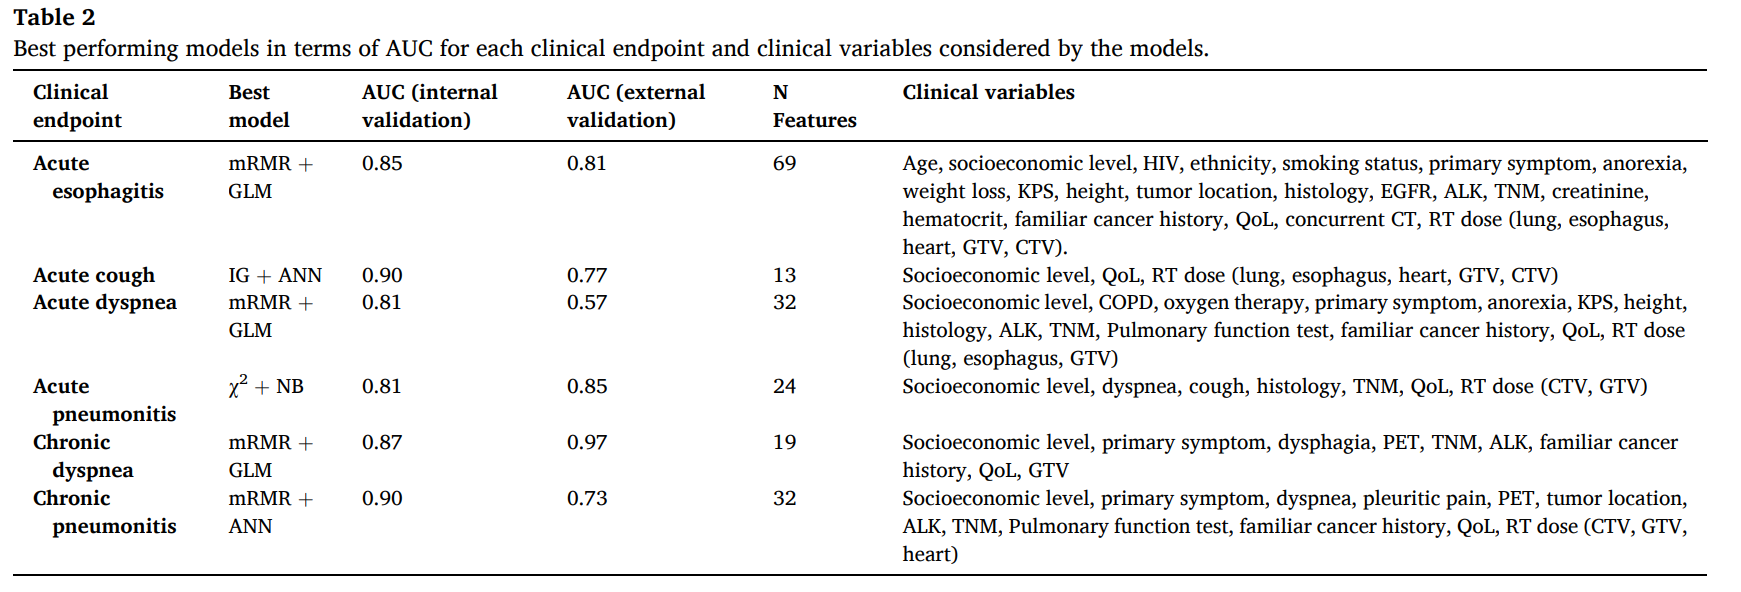
\includegraphics[width=1\textwidth]{tables/nune2023table2.png}
    \captionof{table}{Recopilación de resultados. Extraída de \cite{nunez2023benchmarking}}
    \label{table:nune2023table2}
\end{figure}


\section{Reproducción del estudio con ATLAS} \label{sec:09atlas}
%Caso práctico del TFG

%Check de los casos de uso/requisitos en el estudio real.

- Reinterpretación del estudio

\subsection{Datos}
%\subsection{Comprobación calidad datos}

%- Datos omopizados por TFG Paco 
%- Calidad previa y post comprobada tb en TFG Paco

Se han obtenido el dataset que se utilizó en ese estudio.

- Los datos se convirtieron a OMOP (TFG Paco)

- Se analizó la calidad de los datos eficiente (TFG Paco)

\subsection{Metodología}


\subsubsection{Reporte del dataset}

\subsubsection{Definición de grupos de conceptos}

\subsubsection{Definición de cohortes}

Necesario para utilzar ATLAS

Cohorte = Personas con cancer de pulmon

\subsubsection{Caracterización}

Para conocer los pacientes que tenemos en el cohorte

\subsubsection{Estimación a nivel de población}

Hacer un estudio sobre los efectos adversos que sufrirá la población del cohorte

\subsubsection{Predicción a nivel de Paciente}

Para un paci

\subsection{Resultados}


\section{Discusión de resultados} \label{sec:09resultados}

%Aqui son resultados concretos del estudio. En la sección de resultados serán resultados compeltos del TFG

Comparación de los resultados obtenidos en el estudio del HUVR y el estudio realizado con ATLAS


\section{Conclusiones} \label{sec:09conclusiones}

En este capítulo se concluye que...